\documentclass[10pt, pscyr, nonums]{hedlabwork}
\usepackage[russian]{babel}
\usepackage{hedmaths}
\usepackage{graphicx}
\graphicspath{{images/}, {plots/}}

\newgeometry{top=1.5cm, bottom=1.5cm, left=1cm, right=1cm}

\student{Слоква В. И., Ф-469}
\date{18.09.2013}
\labnum{501}
\labname{Определение постоянной Стефана-Больцмана
при помощи оптического пирометра}

\begin{document}
    \makeheader

    \emph{Цель работы:} изучение законов теплового излучения и
    экспериментальное определение постоянной Стефана-Больцмана при помощи
    оптического пирометра.
    
    \emph{Используемые при расчетах формулы и значения:}
    \( S = 2,3\cdot10^{-5}~\text{м}^2; \ \sigma = \cfrac{JU}{S(T^4 - T_0^4)};
    \ T = t + 273 \).

    \begin{figure}[h!]
        \center
        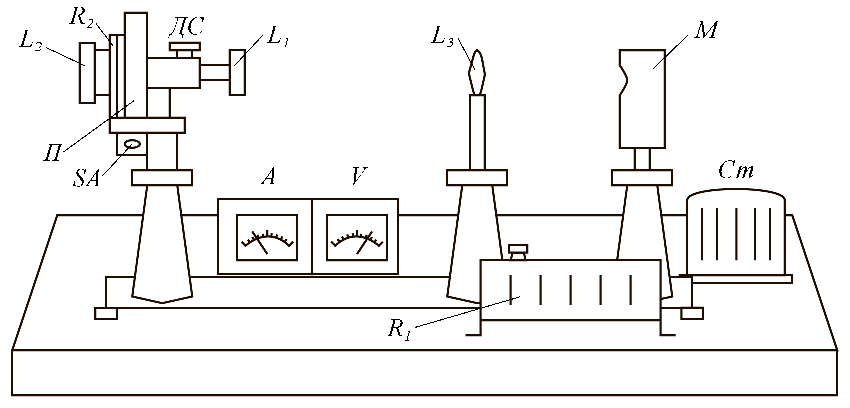
\includegraphics[width=.4\textwidth]{appearance} \hspace*{2em}
        
\includegraphics[width=.4\textwidth]{scheme} \\[.5em]
        \parbox{.4\textwidth}{\caption{Внешний вид установки}} \hspace*{2em}
        \parbox{.4\textwidth}{\caption{Принципиальная схема}}
    \end{figure}
    \vspace*{-2em}
    
    \begin{table}[h!]
        \center \caption{Результаты измерений и вычислений постоянной
        Стефана-Больцмана}
        \begin{tabular}{|*{9}{C{.08}|}} \hline
            \multicolumn{5}{|c|}{Температура} &
                \multirow{3}{*}{Ток \( J \)} &
                \multirow{2}{*}{Напря-} &
                \multirow{3}{*}{\( \sigma \)} &
                \multirow{3}{*}{\( \midnum{\sigma} \)} \\ \cline{1-5}
            яркостная \( t_s \) & истинная \( t \) &
                истинная \( T \) & воздуха \( t_0 \) &
                воздуха \( T_0 \) &&
                жение \( U \) && \\ \hline
            \( \vphantom{C}^{\circ}\!C \) &
                \( \vphantom{C}^{\circ}\!C \) &
                \( K \) & \( \vphantom{C}^{\circ}\!C \) &
                \( K \) & \( A \) & \( B \) &
                \( \cfrac{10^{-8} \text{Вт}}{\text{м}^2K^4} \) &
                \vspace*{.15em}\( \cfrac{10^{-8}\text{Вт}}{\text{м}^2K^4} \)
                \\[.5em] \hline
            1200 & 1283 & 1556 &
                \multirow{6}{*}{25}  &
                \multirow{6}{*}{298} &
                3,3 & 5,20 & 10,27 &
                \multirow{6}{*}{11,42} \\
            1300 & 1394 & 1667 &&& 3,5 & 5,50 & 10,45 & \\
            1400 & 1508 & 1781 &&& 4,1 & 6,60 & 11,70 & \\
            1500 & 1621 & 1894 &&& 4,4 & 7,25 & 10,78 & \\
            1600 & 1736 & 2009 &&&
                ---\!---\!--- & ---\!---\!--- & ---\!---\!--- & \\
            1700 & 1851 & 2124 &&&
                ---\!---\!--- & ---\!---\!--- & ---\!---\!--- & \\ \hline
        \end{tabular}
    \end{table}
\end{document}
